\documentclass[11pt]{article}

\usepackage{float}
\usepackage[T1]{fontenc}
\usepackage[left=12mm,
right=12mm,top=1.0in,
bottom=1.5in]{geometry}
\usepackage{amsmath}
\usepackage{hyperref}
\usepackage{mathtools}
\usepackage{cancel}
\usepackage{graphicx}
\usepackage{grffile}
\usepackage{caption}
\setcounter{section}{-1}
\graphicspath{{/home/piotr/Documents/database-project/src/jpg/}}
\DeclareUnicodeCharacter{2212}{-}

\begin{document}
\title{{Bazy Danych}}
\author{Projekt\\Piotr Popis\\ 245162}
\date{6 styczen 2020}
\maketitle
\centering
\begin{flushleft}
\section{Przeznaczenie}
Aplikację można wykorzystać w różny sposób. Może być to wirtualny system  postaci lub wykrozystywany do różnorodnych symulacji lub jako np gra. Aplikacja okienkowa zostania napisana w języku Java i zostnie połączona  z relacyjną bazą danych MySQL. Aplikacja będzie się składać z różnych podsystemów, funkcjonalności: \\Systemu logowania,\\
Systemu rejestracji,\\
System pracy,\\
System ekwipunku,\\
System zdobywania surowców\\
Gracz przy rejestracji, będzie wybierał klasę postaci. Następnie będzie komplementował swój ekwipunek zdobywająć surowce np drewno czy złoto. Tym lepszy ekwipunek uzyska tym więcej jest w stanie zdobyć surowców. Zostanie również zaimplementowany ranking graczy(<-ogólnie).
\section{Typy}
Uwzględniam różne typy rejestrowanych kont. Może być to Admin, User lub UserVIP. Konkretne tabele opisze w kolejnych sekcjach.
\subsection{Admin}
Na podstawie klauzuli DELETE będzie mógł usuwać konta poszczególnych graczy jeśli uzna, że doszedł do swojego majątku w sposób niedozwolony.
\\Korzystać z przeglądania wszystkich tabel używając SELECT
\\Będzie mógł modyfikowaC surowce, przedmioty i zmieniać  ekwipunek  gracza dzięki klauzulom ALTER TABLE i update, np nagroda za 1 miejsce w rankingu.
\\Prawo do dodawania kont dzięki klauzuli INSERT, w tej grze kolejnego admina może dodać tylko inny Admin. Oraz nie ma headAdminów. Ich permisje są równe.
\\Używając INSERT INTO będzie miał prawo dodawać nowe wyposażenie, do możliwych dostępnych broni.
\\Usuwanie przedmiotów

\subsection{User}
Użytkownik będzie miał dostęp do klauzuli SELECT, ponieważ musi przeglądać swój ekwipunek i ekwipunek możliwy do zdobycia.
\\ jeśli spełni warunki będzie mógł wykorzystać update do zmiany swojego przeedmiotu.( chociaż nie wiem czy tutaj nie będzie tego sprawdzał admin na podstawie otrzymanych zapytań i akceptował je bądź nie zobacze  co jest bardziej optymalne)

\subsection{UserVIP}
Użytkownik będzie miał dostęp do klauzuli SELECT, ponieważ musi przeglądać swój ekwipunek i ekwipunek możliwy do zdobycia.
\\ jeśli spełni warunki będzie mógł wykorzystać update do zmiany swojego przedmiotu.( chociaż nie wiem czy tutaj nie będzie tego sprawdzał admin na podstawie otrzymanych zapytań i akceptował je bądź nie zobacze  co jest bardziej optymalne).
\\Jako, że jest vipem będzie otrzymywał więcej surowców w wyniki wypraw czy polowań.

\section{Tabele}
Nie wykluczam, że w celu ulepszenia całej aplikacji chciałbym dodać więcej np części ekwipunku typu buty naszyjniki itp. Struktura zostanie przedstawiona na końcu 
\subsection{armors}
W tabeli armors znajdziemy wszystkie dostępne dodane przez Administratorów zbroje wraz z inexami po prostu wygodniej się na nich pracuje i szybciej. 
\subsection{helmets}
W tabeli helmets znajdziemy wszystkie dostępne dodane przez Administratorów zbroje wraz z inexami po prostu wygodniej się na nich pracuje i szybciej. 
\subsection{weapons}
W tabeli weapons znajdziemy wszystkie dostępne dodane przez Administratorów zbroje wraz z inexami po prostu wygodniej się na nich pracuje i szybciej. 
\subsection{shields}
W tabeli shields znajdziemy wszystkie dostępne dodane przez Administratorów zbroje wraz z inexami po prostu wygodniej się na nich pracuje i szybciej. 
\subsection{users}
Tabele przechowuje login oraz hash hasła konkretnego użytkownika znajdujemy w niej też typ oraz unikalny numer konta użytknownika.
\subsection{heroes}
Tabele przechowuje informacje o herosach w bazie. Kazdy heros ma id konta, do ktorego należy , klasę postaci np wojownik oraz odwolanie do posiadanej konfiguracji ekwipunku.
\subsection{equipment}
Zawiera id herosa i indeksy wszystkich przedmiotow ekwipunku czyli na ten moment czworki np (1,2,3,4) Zwykla zbroja , Srebrne Buty, Zlota Tarcza, Platynowy Helm itd. 
\section{Triggery i procedury}
 ON INSERT na users sprawdza czy login jest zajety
\\ ON insert na users sprawdza haslo czy poprawne.
\\ON DELETE na weapons czy jakis gracz nie ma przypadkiem broni ktora chcemy usunac.
\\ON DELETE na, helmets czy jakis gracz nie ma przypadkiem helmu, ktory chcemy usunac.
\\ON DELETE na shields czy jakis gracz nie ma przypadkiem tarczy, ktora chcemy usunac.
\\ON DELETE na armors czy jakis gracz nie ma przypadkiem zbroi, ktora chcemy usunac.
\\ON UPDATE na equipment, czy heroes ma wystarczajaca ilosc zasobow aby zmienic eq na lepsze.
\\ON INSERT na heroes, zeby dodal standardowe startowe przedmioty dla odpowiedniej klasy
\\ON update na equipment, zeby sprawdzil czy odpowiednia klasa zaklada odpowiednie przedmioty
\\Procedura dodania standardowych eq dla klasy
\\ procedura dodawania zlotej,srebrnej,zwyklej,patynowej broni, zbroi, tarczy, helmu
\\procedura do wynagrodzenia pierwszego gracza w rankingu
\\ Chciałbym też podkreślić, że wiele pomysłów pojawia się w czasie implementacji i to na pewno nie są wszystkie urozmaicenia.
\newpage
\section{UML}
Chciałbym podkreślić, że w razie dalszej (np nie ma jeszcze tabeli z rankingiem) implementacji może się zdarzyć, że utworzę więcej tabeli, ale nie zmieni to bardzo samej struktury UML
\begin{figure}[!htbp]
  \begin{minipage}[b]{1.0\textwidth}
    \centering
    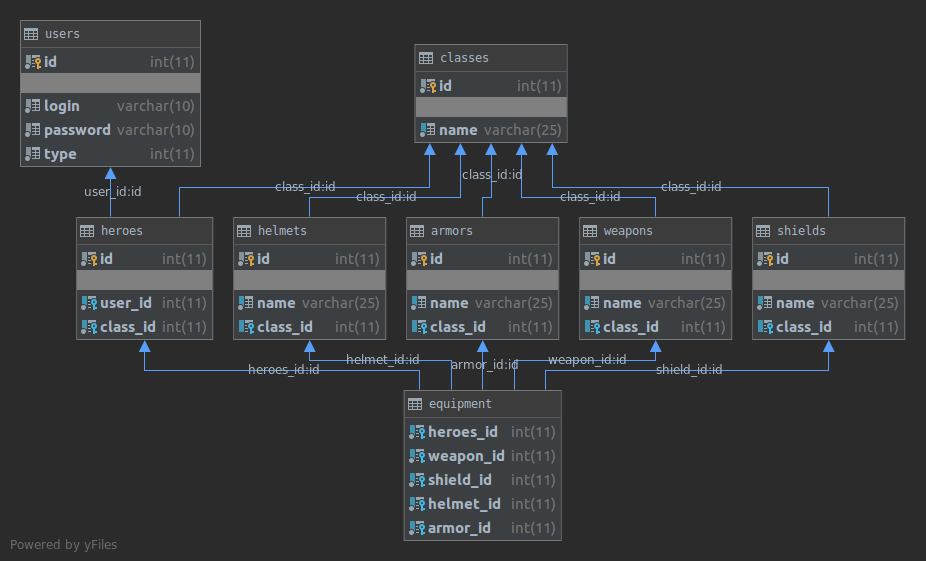
\includegraphics[width=1.0\linewidth]{project.png}
      \end{minipage}\hfill
\end{figure}
\section{modele 3D postaci}
\begin{figure}[!htbp]
\begin{minipage}[b]{1.0\textwidth}
    \centering
    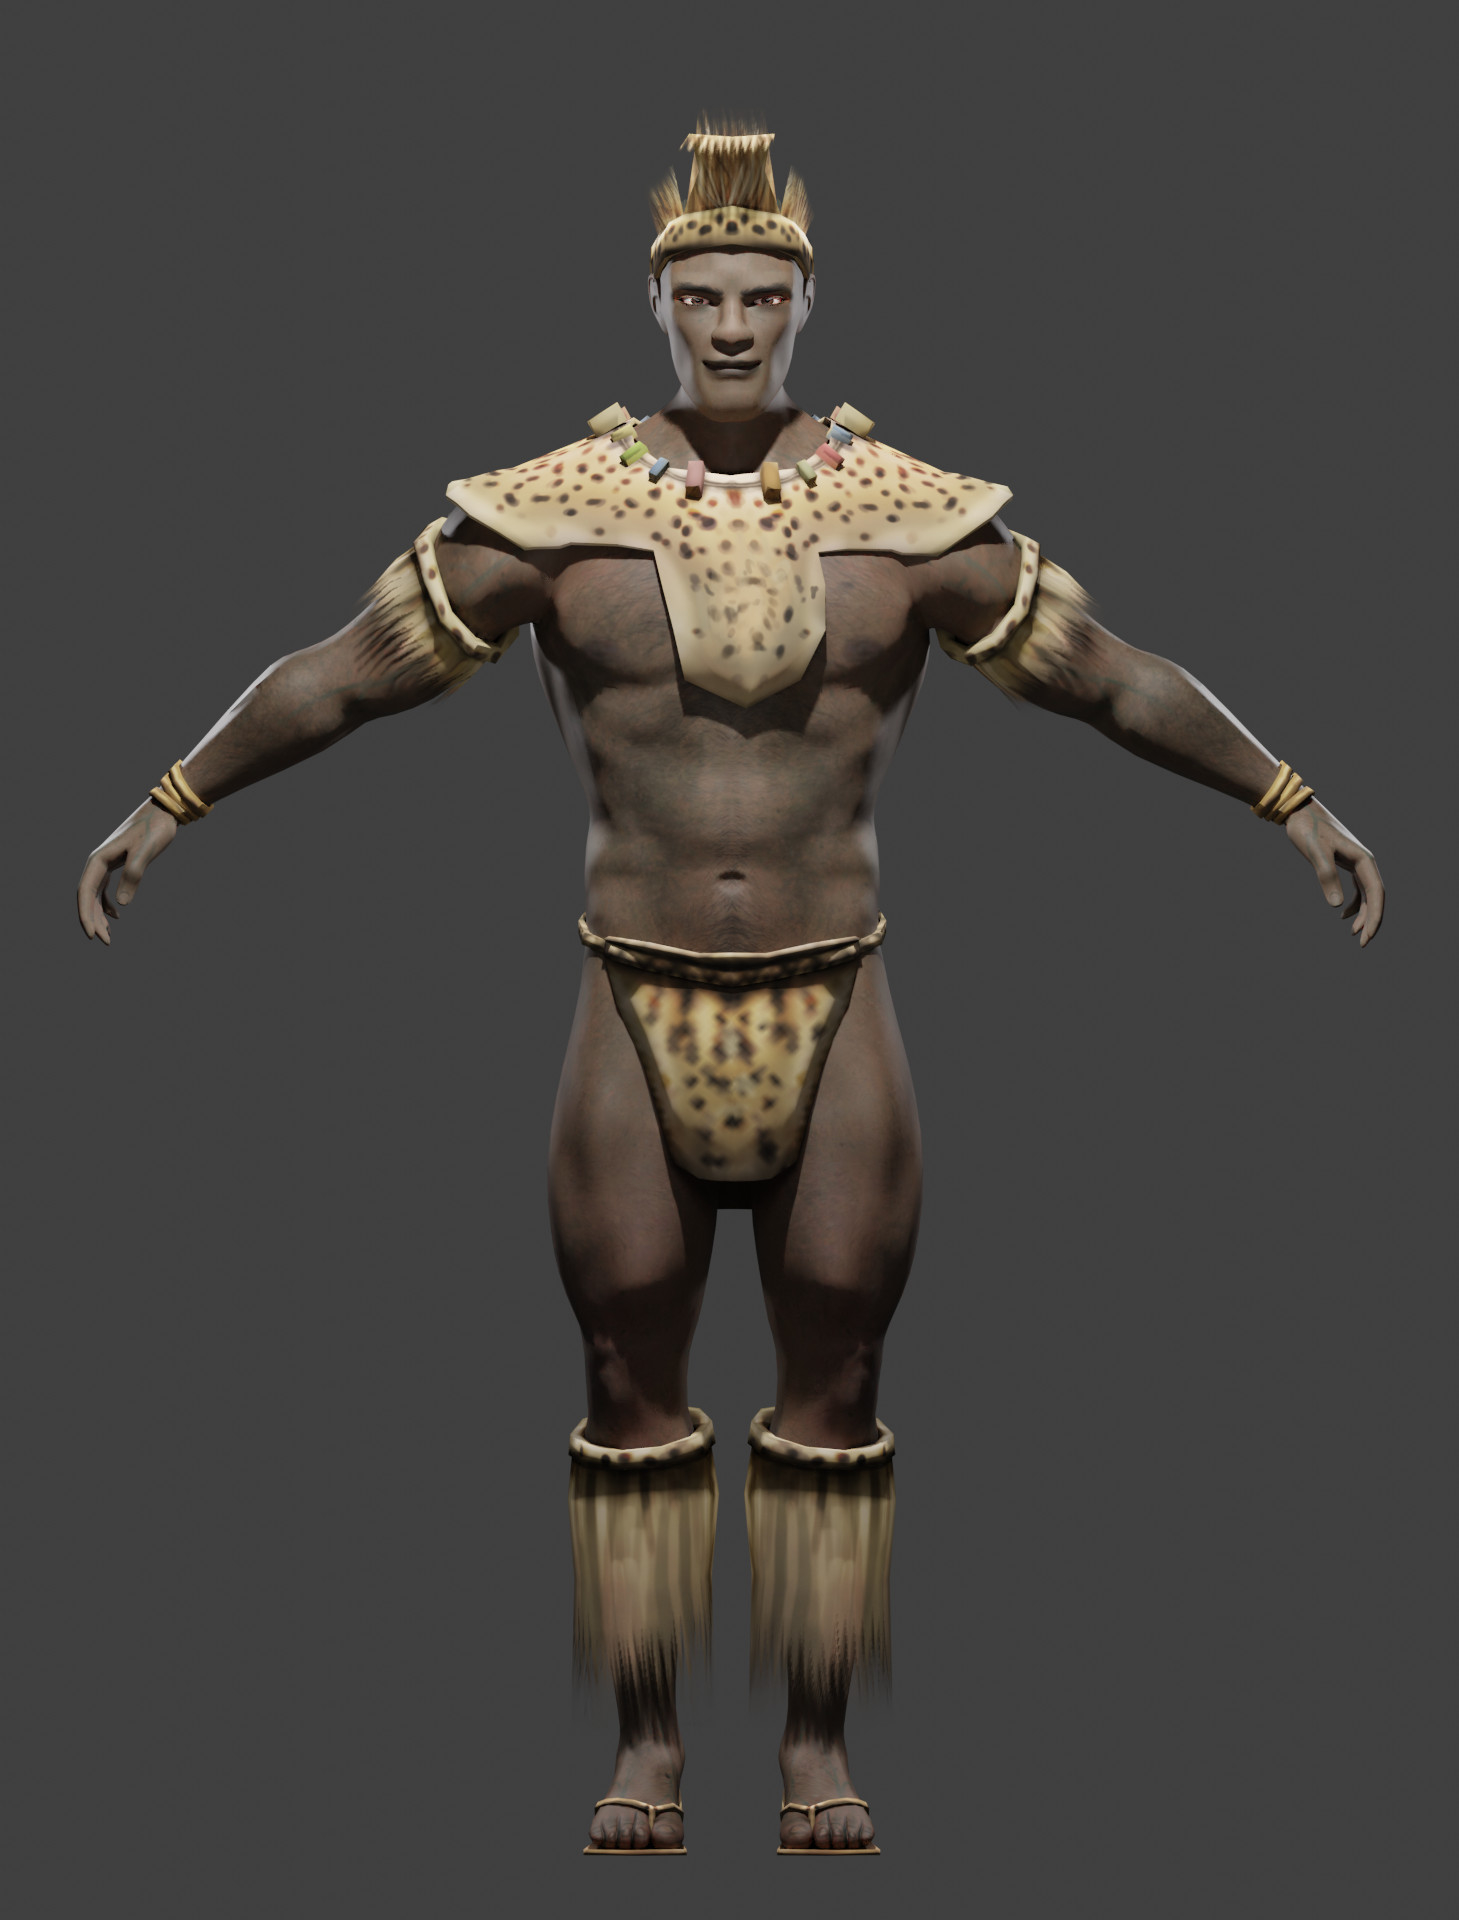
\includegraphics[width=.3\linewidth]{warrior.jpg}
  \end{minipage}\hfill
      \begin{minipage}[b]{1.0\textwidth}
    \centering
    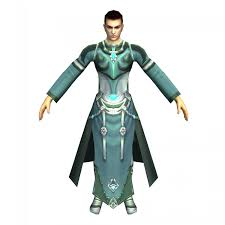
\includegraphics[width=.4\linewidth]{mage.jpeg}
  \end{minipage}\hfill
      \begin{minipage}[b]{1.0\textwidth}
    \centering
    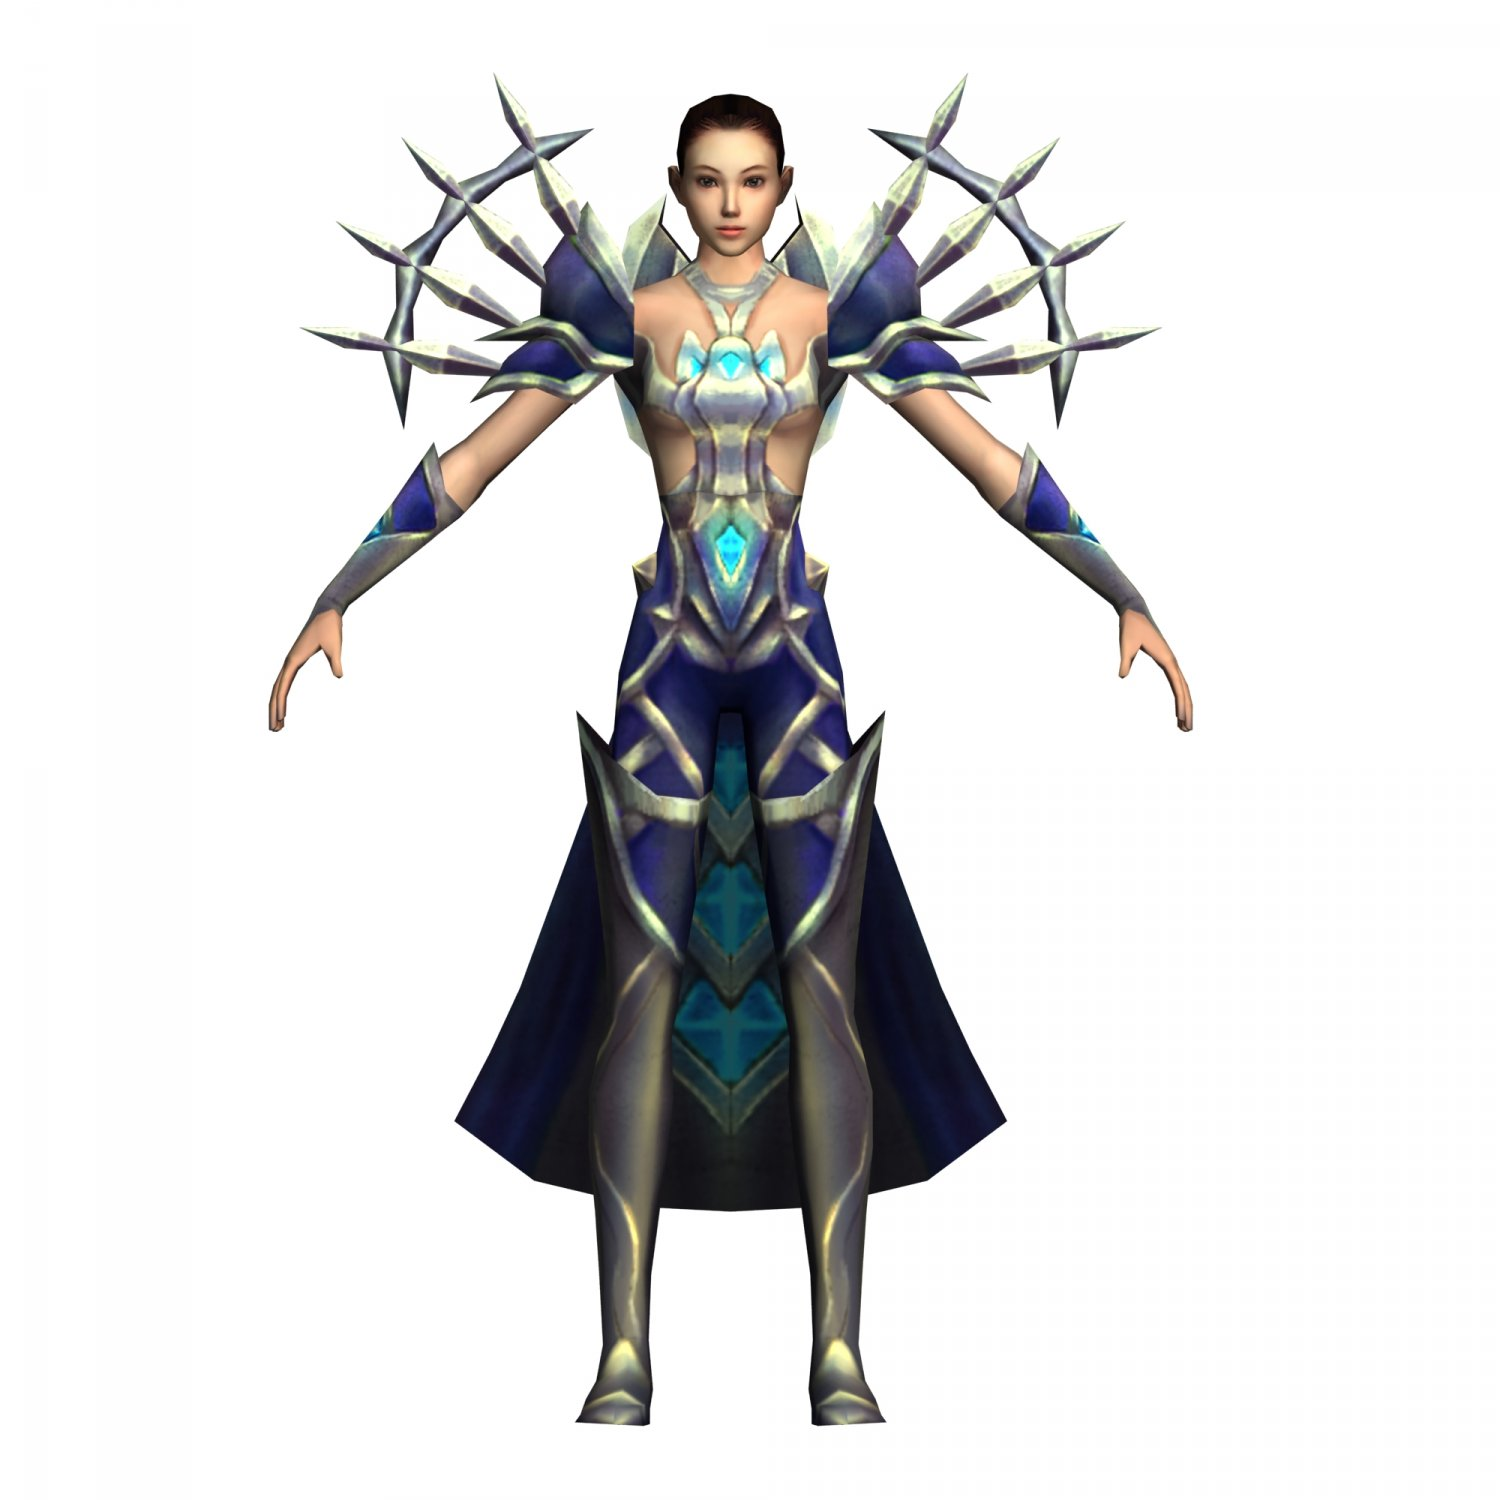
\includegraphics[width=.4\linewidth]{archer.jpg}
  \end{minipage}\hfill
\end{figure}
\section{projekt interfejsu graicznego}
\begin{figure}[H]
\begin{minipage}[b]{1.0\textwidth}
    \centering
    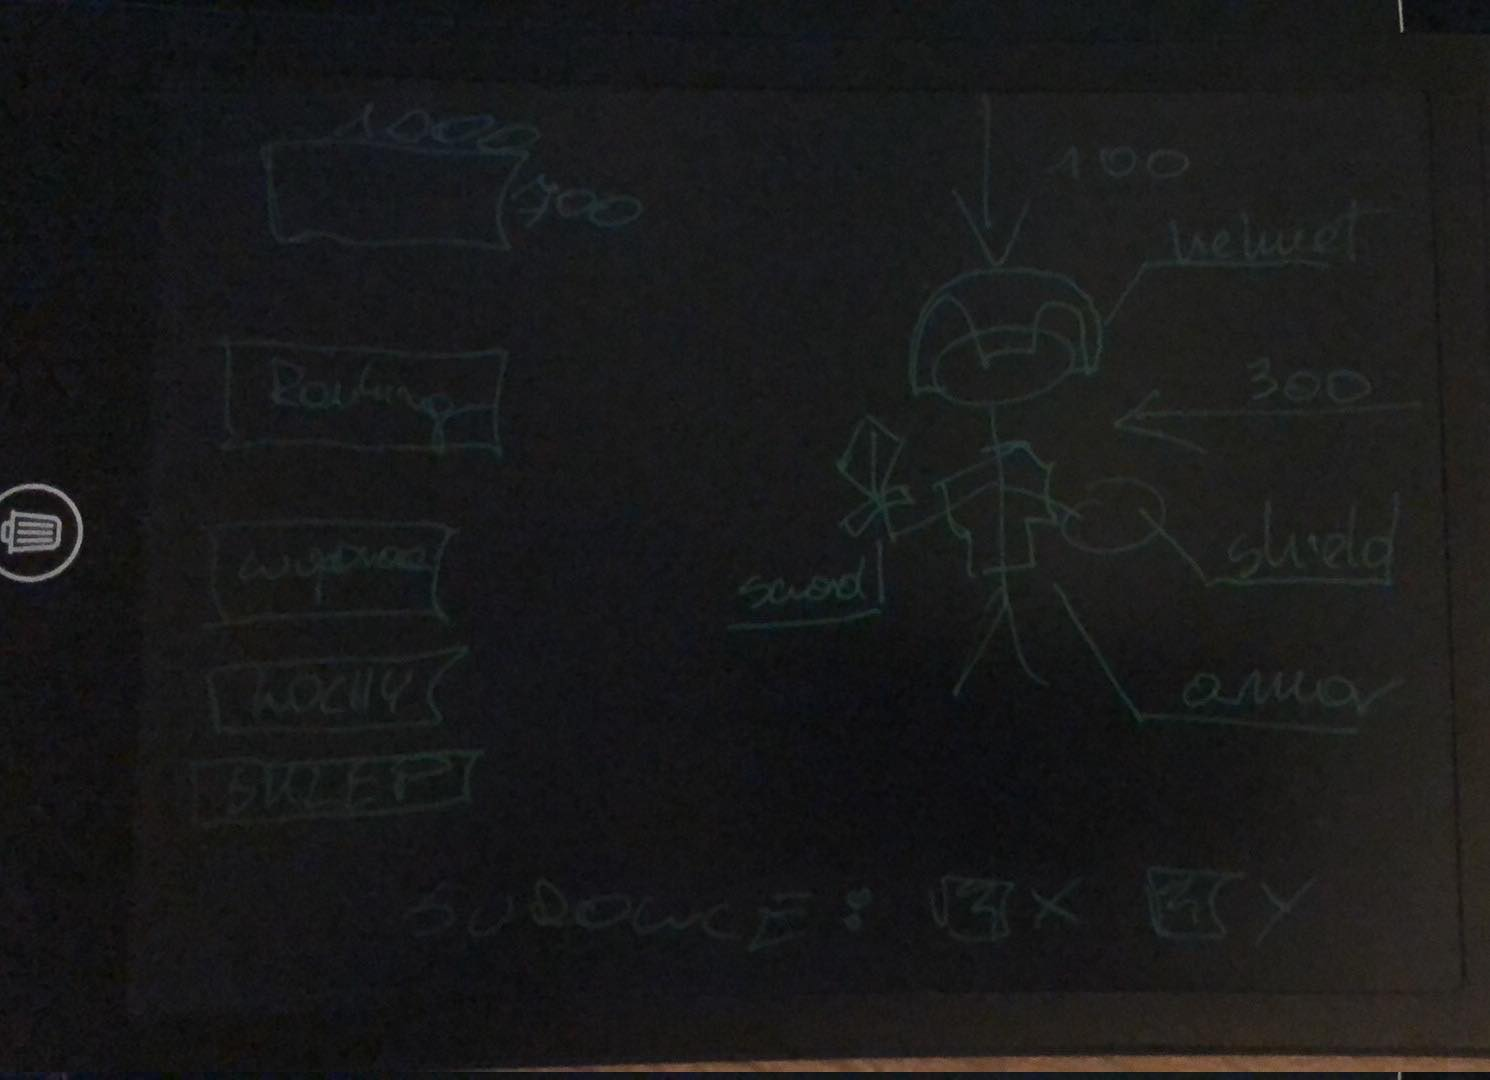
\includegraphics[width=1.0\linewidth]{speculations.jpg}
  \end{minipage}\hfill
\end{figure}
\section{Załączniki}
Dotychczasowy postęp:\\
\href{https://github.com/sqoshi/database-project}{project-git-CLICK!} 
\end{flushleft}
\end{document}